\documentclass[letterpaper,11pt]{article}
\usepackage{standalone}
\usepackage[spanish]{babel}
\usepackage[utf8]{inputenc}
\usepackage[binary-units]{siunitx}
\usepackage{amsmath, amssymb}
\usepackage{ mathrsfs }
\usepackage[left=2.5cm, top=2.5cm, right=2.5cm, bottom=3cm]{geometry}
\usepackage{lastpage}
\usepackage{fancyhdr}
\usepackage{multicol}
\usepackage{hyperref}
\usepackage{color}
\usepackage[binary-units]{siunitx}
\usepackage[american,siunitx]{circuitikz}
\usepackage{placeins}
\usepackage[shortlabels]{enumitem}
\newcommand{\unidad}[1]{\,\si{#1}}
\usepackage{caption}
\usepackage{subcaption}
\captionsetup{justification=centering}
\definecolor{aliceblue}{rgb}{0.94, 0.97, 1.0}
\definecolor{mygreen}{rgb}{0.40, 0.67, 0.3}
\definecolor{antiquewhite}{rgb}{0.98, 0.92, 0.84}
\usepackage{listings}
\usepackage{lstautogobble} % Fix relative indenting
\renewcommand{\lstlistingname}{Listado}
\lstset{
	backgroundcolor={\color{aliceblue}},basicstyle={\small \ttfamily},breaklines=true,captionpos=b,commentstyle={\color{mygreen}},emph={[1]{for,end,break}},emphstyle={[1]\color{red}},frame=tb,identifierstyle={\color{black}},keywordstyle={\color{blue}},language=scilab,morekeywords={[2]{1}},numbers=left,numbersep=9pt,numberstyle={\tiny \color{black}},showstringspaces=false,stringstyle={\color{red}}}

\fancyfoot[C]{\thepage\ de \pageref{LastPage}}

\begin{document}
	\thispagestyle{empty}
	% MATERIA
\newcommand{\materia}{\uppercase{Control I}}
% MAESTRO
\newcommand{\maestro}{\uppercase{Gerardo Marx Chavez Campos}}

% TIPO DOCUMENTO
\newcommand{\tipoDoc}{\uppercase{REPORTE DE LABORATORIO}} %TAREA, REPORTE DE LABORATORIO,
% NOMBRE DE DOCUMENTO
\newcommand{\nombreDoc}{\uppercase{Práctica 1}} 
% NUMERO DE DOCUMENTO (SI ES NECESARIO)
\newcommand{\docNum}{}
% SUBNOMBRE DOCUMENTO
\newcommand{\subNombreDoc}{\uppercase{Analisis de un sistema de primer orden}}

% ALUMNOS 
\newcommand{\alumnos}{\uppercase{GABRIEL AGUILAR LEMUS \\ José Pablo Barragán Franco}}
% FECHA DE ENTREGA
\newcommand{\fecha}{\uppercase{28 de octubre de 2017}}

\begin{center}
	\
	\includegraphics[scale=.5]{/home/gabriel/LATEX/PortadaOficial/encabezado.png}
	\huge INSTITUTO TECNOLÓGICO DE MORELIA \\
	\vfill
	\large DIVISIÓN DE ESTUDIOS PROFESIONALES  \\
	\vfill
	\large  DEPARTAMENTO DE INGENIERÍA ELECTRÓNICA \\ 
	\vfill
	\Large \textbf \materia \\
	\vfill
	\textbf{\tipoDoc} \\
	\vfill 
	\LARGE  \textbf{ \nombreDoc  \, \docNum: \\ \subNombreDoc} \\
	\vfill
	\large PRESENTA(N): \\
	\LARGE  \textbf{\alumnos} \\
	\vfill
	\large PROFESOR(A): \\
	\Large \textbf{\maestro }
	\vfill 
	\begin{flushleft}
		MORELIA, MICHOACÁN \hfill \uppercase{\fecha}
	\end{flushleft}
	\pagebreak
\end{center}
	\thispagestyle{plain}
	\section{Introducción}
	Una función de transferencia es la relación entre la entrada y la salida de un sistema y(s), u(s) ambas se pueden expresar en el dominio del tiempo y(t), u(t)  o de frecuencia aplicando transformadas de Laplace se obtiene $Y(s)$, $U(s)$ y existe un $G(s)$ que es el encargado de relacionar la entrada y la salida.
	\begin{figure}[h!]
\centering
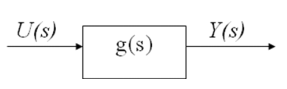
\includegraphics[scale=1]{screenshot001}
\caption{Función de transferencia}
\label{fig:screenshot001}
\end{figure}

	Se puede representar cualquier sistema mecánico, térmico, hidráulico con una función de transferencia que a su vez se puede trasladar a un modelo eléctrico para una mayor comprensión y así poder trabajar de una manera más sencilla sobre este sistema modificar parámetros y valores para obtener la respuesta correcta del sistema.\\
	Los sistemas contienen constantes que determinan su comportamiento y la constante temporal $\tau$ establece el tiempo en el que un sistema reacciona a un cambio.
	\section{Metodología}
	El análisis de un sistema de primer orden involucra la respuesta de la función de transferencia del tipo
	\[H(s)=\frac{bs+c}{s+a}\]
	en donde los elementos de una fracción de funciones lineales describen el comportamiento de un sistema que se modela dando valores a las constantes de la ecuación.\\
	Sin embargo en la realidad es conveniente analizar la respuesta forzada de un sistema, usualmente en forma de la respuesta al escalón unitario. Este estímulo se representa matemáticamente de la siguiente manera
	\[H_{step}(s) = \frac{1}{s} H(s)\]
	Para realizar el análisis se reescribe la ecuación anterior en su equivalente en fracciones parciales realizando el procedimiento que a continuación se describe.\\
	Tenemos una expresión fraccionaria del tipo
	\[\frac{P_n}{P_m}\]
	donde $m > n$. \\
	Para simplificar la función de transferencia se establece la igualdad
	\[\frac{bs+c}{s\left(s+a\right)} = \frac{A}{s} + \frac{B}{s+a}\]
	multiplicando la ecuación por $s\left(s+a\right)$ se tiene
	\[bs+c = A\left(s+a\right) +Bs\]
	lo cual propone el sistema de ecuaciones\\
	\[
	\begin{cases}
	 A+B=b\\
	 aA=c
	\end{cases}
	\]
	por simple inspección se determina que
	\[A = \frac{c}{a}\qquad B=\frac{ab-c}{a}\]
	Lo que completa la expresión de la función de transferencia de un sistema genérico de primer orden
	\[H(s)=\frac{c}{as}+\frac{ab-c}{a\left(s+a\right)}\]
	Para continuar con el análisis de la función de transferencia de primer orden es necesario encontrar su forma en el dominio del tiempo. Esto se logra aplicando a la función la transformada inversa de Laplace.
	\[\mathscr{L}^{-1} H(s) = \mathscr{L}^{-1}\left(\frac{c}{as}+\frac{ab-c}{a\left(s+a\right)}\right) \]
	La respuesta temporal del sistema tiene la forma
	\[h(t)=\frac{c}{a}\mathscr{U}\left(t\right)+\frac{ab-c}{a}e^{-at}\]
	Donde para $t > 0$
	\[h(t)=\frac{c}{a}+\frac{ab-c}{a}e^{-at}\]
	En el siguiente listado se muestra una función de Scilab donde se introducen las constantes de un sistema de primer orden y se obtiene en la salida una gráfica de su respuesta temporal.
	\lstinputlisting[label={lst:codigo1},caption={Procedimiento de Scilab donde se introducen los coeficientes de la función de transferencia de un sistema de primer orden.}]{../first-order-systems-aguilar_barragan/uStpRes.sce} 
	El código del listado \ref{lst:codigo1} grafica la respuesta temporal del sistema a partir de los términos obtenidos del análisis de su función de transferencia. Sin embargo el código brindado para la práctica, mostrado en el listado \ref{lst:codigoMarx}, efectuá los calculos necesarios para obtener la respuesta temporal a partir de la función de transferencia.
	\lstinputlisting[label={lst:codigoMarx},caption={Código brindado por el profesor.}]{../first-order-systems-aguilar_barragan/firstOrderSystem.sce}
	Los calculos necesarios son efectuados por funciones pertenecientes al entorno de Scilab.
	\subsection{Sistema de primer orden hidráulico}
	
	Como un ejemplo real de un sistema de primer orden se puede considerar el sistema de la figura \ref{fig:tankScheme}.
	\begin{figure}
	\centering
	\includegraphics[width=0.3\linewidth]{../first-order-systems-aguilar_barragan/tankScheme}
	\caption{Esquema de sistema hidráulico}
	\label{fig:tankScheme}
	\end{figure}
	Se considera que el tanque es llenado a un flujo $W_{in} [\frac{m^3}{s}]$, o sea la entrada del sistema. La salida es el flujo de descarga $W_{out} [\frac{m^3}{s}]$. Si $W_{in} = W_{out}$, el nivel $h(t)$ del agua permanece constante. Si $W_{in} > W_{out}$, el nivel del agua crece. Si $W_{in} < W_{out}$, el nivel decrece.
	Para comenzar el análisis de un sistema de cualquier tipo es necesario establecer una relación de energía en el sistema. Dadas las leyes de la termodinámica la energía total de un sistema es igual a la energía introducida al sistema mas la energía entregada por el sistema menos las perdidas. Expresado lo anterior en términos matemáticos
	\[\sum E_{entradas} = \sum E_{salidas} + \sum E_{perdidas}\]
	En nuestro sistema hidráulico lo que se quiere analizar es el nivel de agua en el tanque. Esta altura depende de la cantidad de agua que entra y sale del mismo. Por lo tanto
	\[W_{in} = W_{out} + W_{acc}\]
	el volumen del agua entrante es el mismo que sale mas el volumen acumulado.
	La función temporal de este sistema toma la forma
	\[w_{in}(t) = h(t)\frac{gA_R}{R}+A\frac{dh(t)}{dt}\]
	donde $g$ es la gravedad en la tierra, $A_R$ el área del tubo de salida, $R$ la resistencia al flujo del tubo y $A$ el área del tanque. Al aplicar la transformada de Laplace a la función se tiene
	\[ \mathscr{L}\left( w_{in}(t) = h(t)\frac{gA_R}{R}+A\frac{dh(t)}{dt} \right) \]\\
	\[ W_{in}(s) = H(s) \frac{gA_R}{R} + A\left( sH(s) + h(0) \right)\]
	Considerando un tanque vacío como condición inicial. Para encontrar la función de transferencia dividimos la ecuación por $H(s)$.
	\[ \frac{W_{in}}{H(s)} =\frac{g A_R}{R} +As = \frac{g A_R+ARs}{R} \]
	\[\text{ FT} = \frac{H(s)}{W_{in}(s)} = \frac{R}{g A_R+ARs} \]
	La función de transferencia contiene todos los términos relevantes del sistema para su modelado. El comportamiento del sistema depende de dichas constantes por lo que las condiciones en donde $W_{in} = W_{out}$, $W_{in} < W_{out}$ y $W_{in} > W_{out}$ sucederán en valores específicos de las constantes.
	En el caso de la igualdad de los flujos el término de acumulación del contenedor es cero por lo que se considera que no existe el tanque.
	\[ W_{in}(s) = H(s) \frac{gA_R}{R} \]
	Este caso del sistema puede modelarse eléctricamente como se muestra en el circuito de la figura \ref{fig:cir1}
	\begin{figure}
		\centering
		\begin{tikzpicture}
			\draw
			(0,0) node[ground]{}
			(1,3) to[short,-*] (1,3)
			(1,3.3) node[]{$h(t)$}
			(0,0) to[current source,l=$W_{in}$] (0,3)
			to[short,-|] (2,3)
			to[R,l=$\frac{gA_R}{R}$] (2,0)
			to[short,-*] (0,0)
			;
		\end{tikzpicture}
		\caption{Circuito equivalente al caso $W_{in} = W_{out}$}
		\label{fig:cir1}
	\end{figure}
	En cualquiera de los otros dos casos el nivel del agua dependerá de la condición inicial del tanque y de la resistencia al flujo de salida. Una resistencia muy alta hará que el flujo de entrada sea mayor al de salida provocando un incremento del nivel del agua. Una resistencia muy baja provocara que el flujo de salida sea mas grande que la entrada, generando muy poco almacenaje de agua.
	\section{Resultados y discusión}
	Para comparar las funciones de los listados \ref{lst:codigo1} y \ref{lst:codigoMarx} se ejecutan considerando la siguiente función de transferencia
	\[ F(s) = \frac{1}{1+s}\]
	El resultado de evaluar el sistema anterior en ambas ecuaciones resulta en las gráficas de las figuras \ref{fig:graph1} y \ref{fig:graph2}. Se puede observar que ambas figuras son idénticas, lo que indica que el calculo realizado teóricamente es el mismo que contiene scilab dentro de sus funciones.
	\begin{figure}[h!]
		\centering
		\includegraphics[width=0.7\linewidth]{../first-order-systems-aguilar_barragan/graph1}
		\caption{Gráfica generada por el código de Scilab.}
		\label{fig:graph1}
	\end{figure}
		\begin{figure}[h!]
			\centering
			\includegraphics[width=0.7\linewidth]{../first-order-systems-aguilar_barragan/graph2}
			\caption{Gráfica generada por el código resultado del análisis del sistema.}
			\label{fig:graph2}
		\end{figure}
%	Escribiendo la función de transferencia del sistema hidráulico en la forma genérica se tiene:
%	\[ F(s) = \frac{\frac{1}{A}}{\frac{gA_R}{AR}+s} \]
%	Proponiendo valores a la función de transferencia del sistema hidráulico podemos modelar los casos donde  $W_{in} = W_{out}$, $W_{in} < W_{out}$ y $W_{in} > W_{out}$.\\
%	Para $W_{in} = W_{out}$:
%	\[ F(s) =  \frac{R}{g A_R}\]
	
\section{Conclusiones}
	Los sistemas de primer orden son la fundación de muchos sistemas que utilizamos día a día. Su análisis depende de sencillas relaciones que surgen a partir de la poderosa herramienta de la transformada de Lapĺace. Esta nos abre las puertas a analizar los sistemas mas allá de sus respuestas temporales y permite estudiar muchas características del sistema, desde sus constante temporal $\tau$ hasta la calidad de la respuesta a diferentes frecuencias. Este analisis tan común esta embebido en los software de análisis numérico dada su utilidad y se basan en principios bien conocidos.
\end{document}